%%%%%%%%%%%%%%%%%%%%%%%%%%%%%%%%%%%%%%%%%%%%%%%%%%%%%%%%%%%%%%%%%%
\section{Background: Dynamic Subtree Partitioning}	%%%%%%%%%%
\label{background_dynamic_subtree_partitioning}			%%%%%%%%%%
%%%%%%%%%%%%%%%%%%%%%%%%%%%%%%%%%%%%%%%%%%%%%%%%%%%%%%%%%%%%%%%%%%
\begin{figure}[tb]
	\centering	
	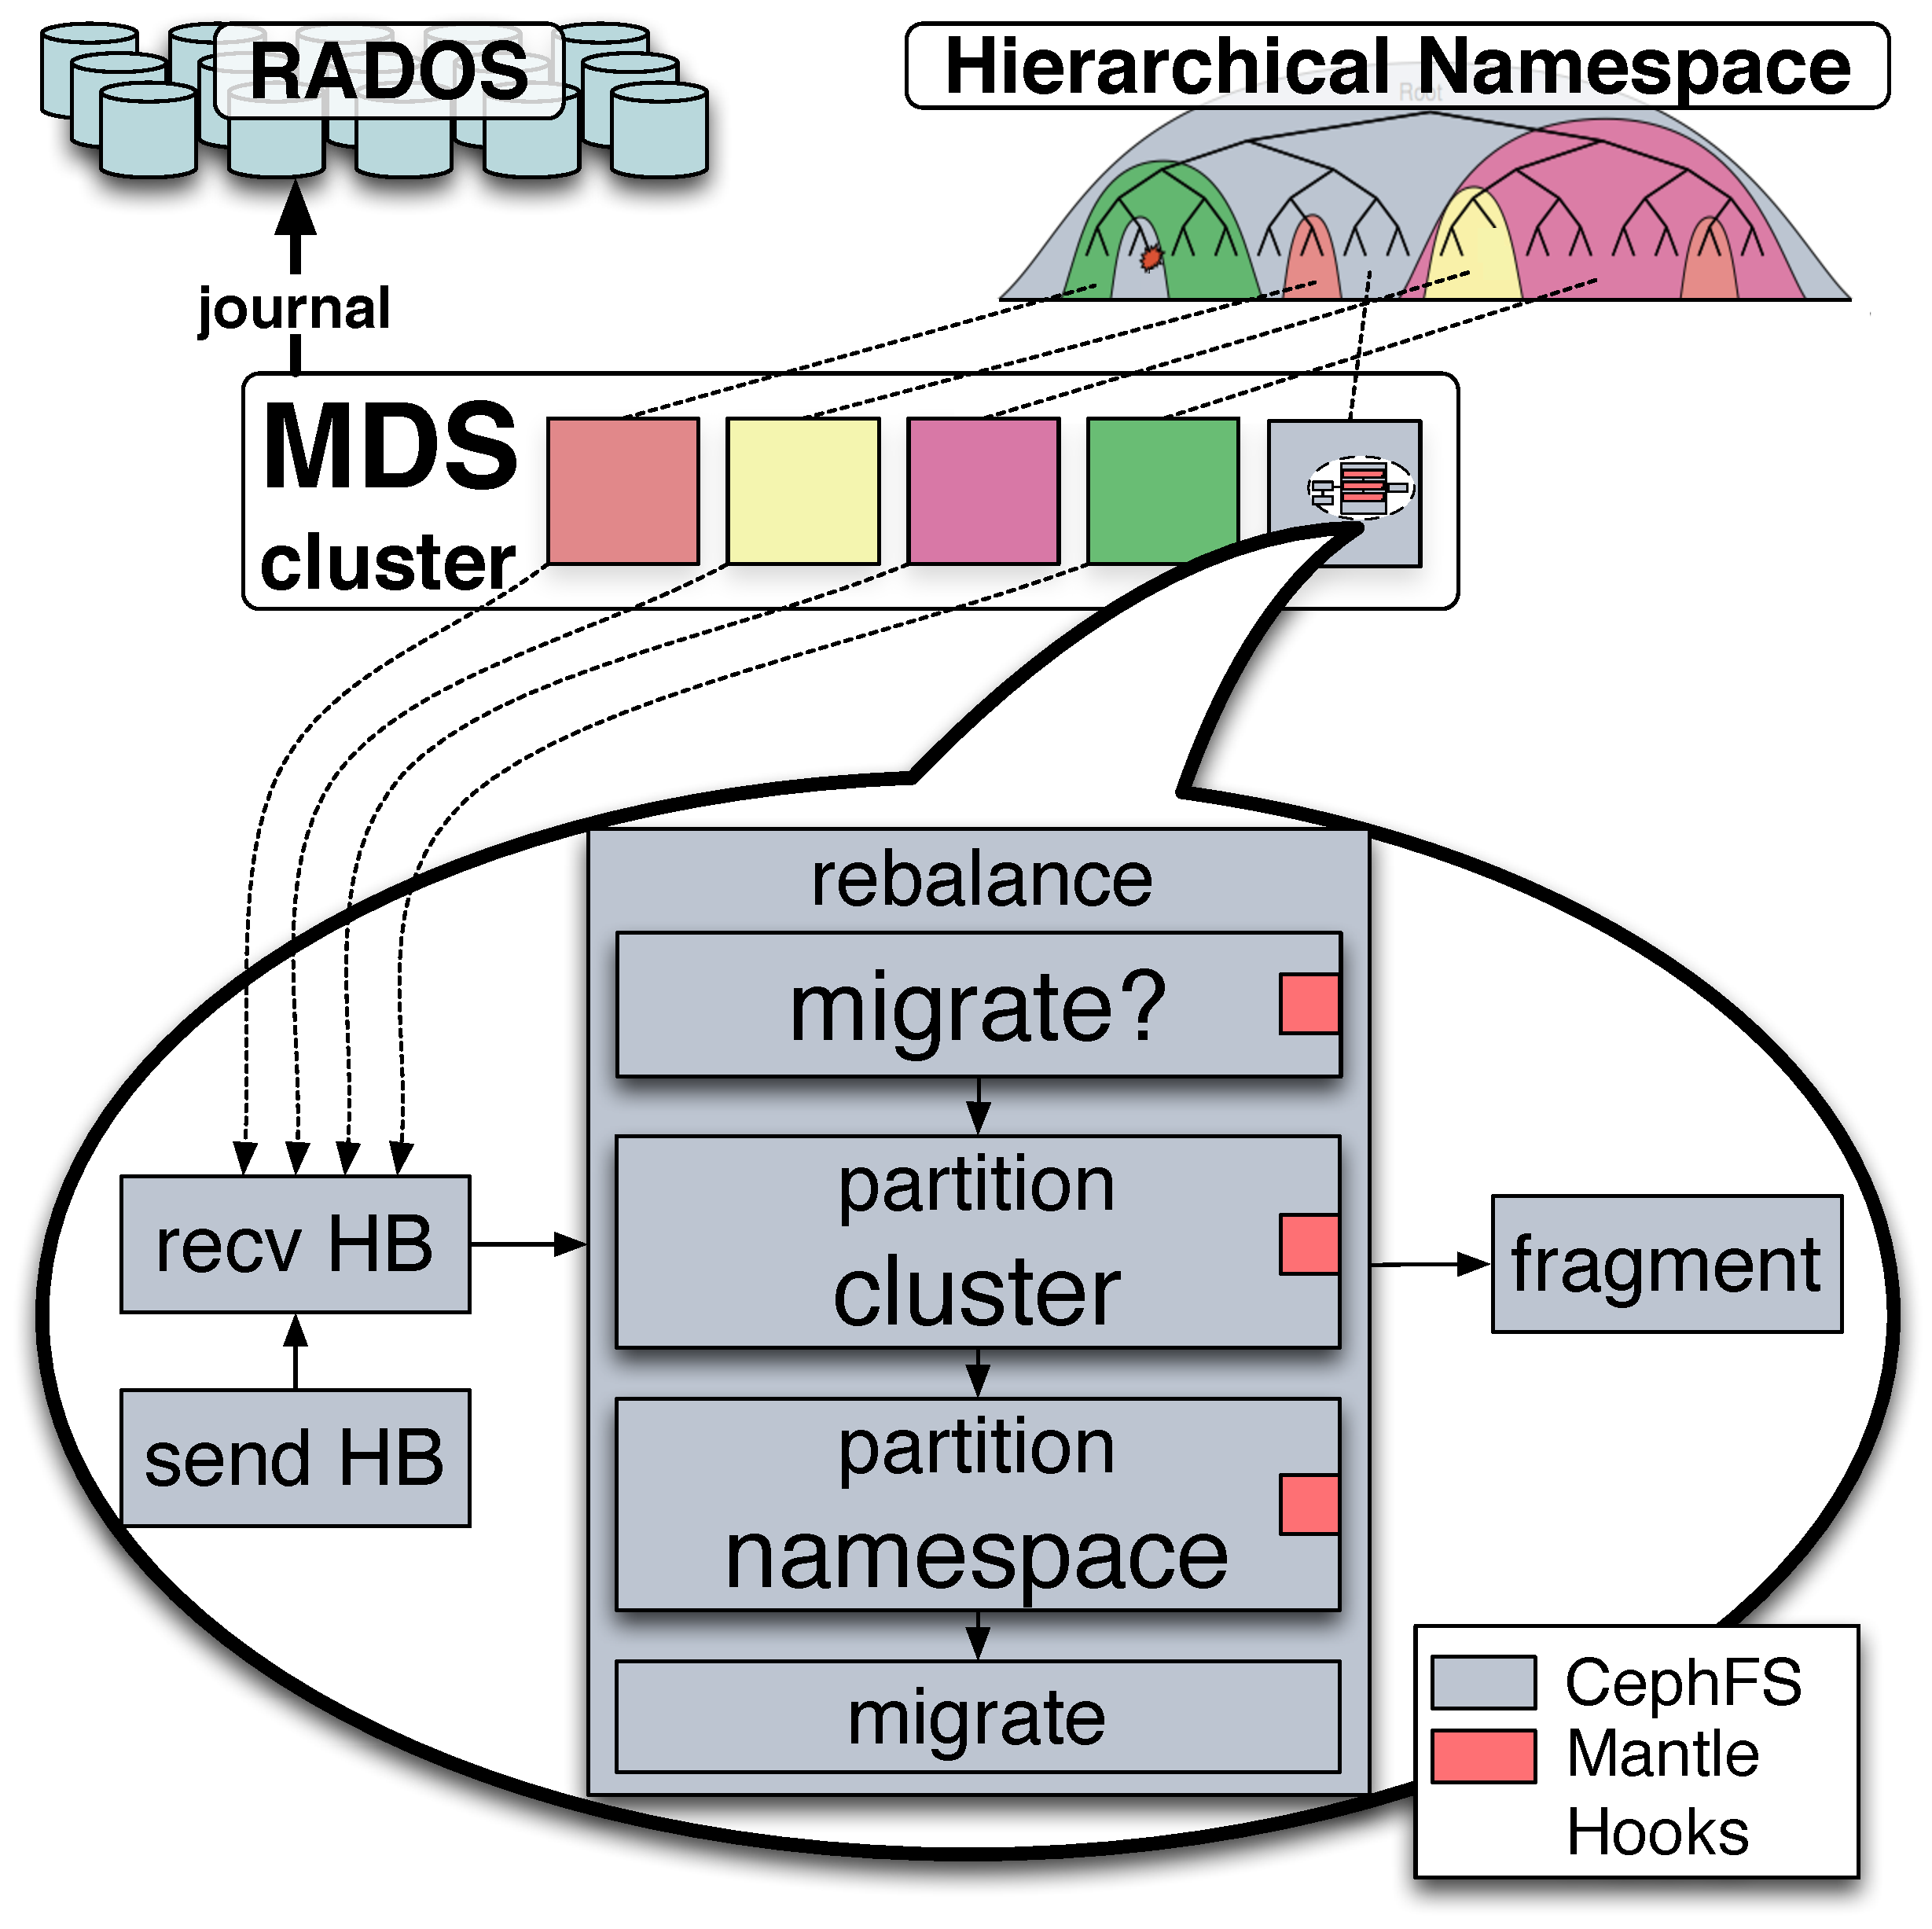
\includegraphics[width=0.4\textwidth]{./chapters/mantle/figures/balancer-diagram.pdf}
 	\caption{The MDS cluster journals to RADOS and exposes a namespace to clients. Each MDS makes decisions by exchanging heartbeats and partitioning the cluster/namespace. Mantle adds code hooks for custom balancing logic.\label{figure:balancer-diagram}}    
\end{figure}   


% Outline of the figure.
In CephFS MDS nodes use dynamic subtree partitioning~\cite{weil:sc2004-dyn-metadata} to carve up the namespace and to distribute it across the MDS cluster, as shown in Figure~\ref{figure:balancer-diagram}. MDS nodes maintain the subtree boundaries and ``forward" requests to the authority MDS if a client's request falls outside of its jurisdiction or if the request tries to write to replicated metadata.  Each MDS has its own metadata balancer that makes independent decisions, using the flow in Figure~\ref{figure:balancer-diagram}.  Every 10 seconds, each MDS packages up its metrics and sends a heartbeat (``send HB") to every MDS in the cluster. Then the MDS receives the heartbeat (``recv HB'') and incoming inodes from the other MDS nodes. Finally, the MDS decides whether to balance load (``rebalance'') and/or fragment its own directories (``fragment"). If the balancer decides to rebalance load, it partitions the namespace and cluster and sends inodes (``migrate'') to the other MDS nodes. These last 3 phases are discussed below.

% Migrate
\textbf{Migrate}: inode migrations are performed as a two-phase commit, where the importer (MDS node that has the capacity for more load) journals metadata, the exporter (MDS node that wants to shed load) logs the event, and the importer journals the event. Inodes are embedded in directories so that related inodes are fetched on a \texttt{readdir} and can be migrated with the directory itself.

% Partitioning the namespace
\textbf{Partitioning the Namespace}: each MDS node's balancer carves up the namespace into {\it subtrees} and {\it directory fragments} (added since~\cite{weil:sc2004-dyn-metadata,weil:osdi2006-ceph}). Subtrees are collections of nested directories and files, while directory fragments ({\it i.e.} dirfrags) are partitions of a single directory; when the directory grows to a certain size, the balancer fragments it into these smaller dirfrags. This directory partitioning mechanism is equivalent to the GIGA+~\cite{patil:fast2011-giga+} mechanism, although the policies for moving the dirfrags can differ.  These subtrees and dirfrags allow the balancer to  partition the namespace into fine- or coarse-grained units.

% How does the balancer partition the namespace: metadata load
Each balancer constructs a local view of the load by identifying popular subtrees or dirfrags using metadata counters. These counters are stored in the directories and are updated by the MDS whenever a namespace operation hits that directory or any of its children. Each balancer uses these counters to calculate a {\it metadata load} for the subtrees and dirfrags it is in charge of (the exact policy is explained in Section~\S\ref{the-cephfs-policies}). The balancer compares metadata loads for different parts of its namespace to decide which inodes to migrate. Once the balancer figures out which inodes it wants to migrate, it must decide where to move them.

% What is partitioning cluster
\textbf{Partitioning the Cluster}: each balancer communicates its metadata load and resource metrics to every other MDS in the cluster. Metadata load metrics include the metadata load on the root subtree, the metadata load on all the other subtrees, the request rate/latency, and the queue lengths. Resource metrics include measurements of the CPU utilization and memory usage. The balancer calculates an {\it MDS load} for all MDS nodes using a weighted sum of these metrics (again, the policy is explained in Section~\S\ref{the-cephfs-policies}), in order to quantify how much work each MDS is doing. With this global view, the balancer can partition the cluster into exporters and importers. These loads also help the balancer figure out which MDS nodes to ``target'' for exporting and {\it how much} of its local load to send. The key to this load exchange is the load calculation itself, as an inaccurate view of another MDS or the cluster state can lead to poor decisions.

\textbf{CephFS's Client-Server Metadata Protocols}: the mechanisms for migrating metadata, ensuring consistency, enforcing synchronization, and mediating access are discussed at great length in~\cite{weil:phdthesis07} and the Ceph source code. MDS nodes and clients cache a configurable number of inodes so that requests like \texttt{getattr} and \texttt{lookup} can resolve locally.  For shared resources, MDS nodes have coherency protocols implemented using scatter-gather processes. These are conducted in sessions and involve halting updates on a directory, sending stats around the cluster, and then waiting for the authoritative MDS to send back new data. As the client receives responses from MDS nodes, it builds up its own mapping of subtrees to MDS nodes. 

%%%%%%%%%%
\subsection{Advantages of Locality}
\label{advantages_of_locality}
%%%%%%%%%%
\begin{figure*}[tbh]
	\begin{subfigure}[H]{0.45\textwidth}
		\centering	
	\caption{The number of requests for the compile job.  \label{figure:workload-tar-requests-total}}
		
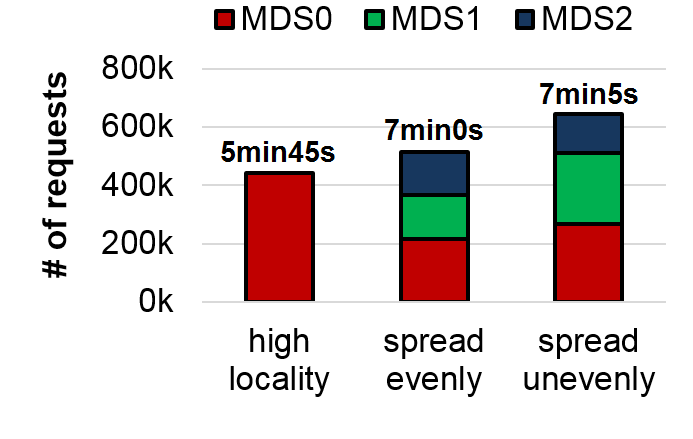
\includegraphics[width=1\textwidth]{./chapters/mantle/figures/workload-tar-requests2.png}
	\end{subfigure}
	~
	\begin{subfigure}[H]{0.47\textwidth}
		\centering
		\caption{Path traversals ending in hits (local metadata) and forwards. \label{figure:workload-tar-traverses}}	
	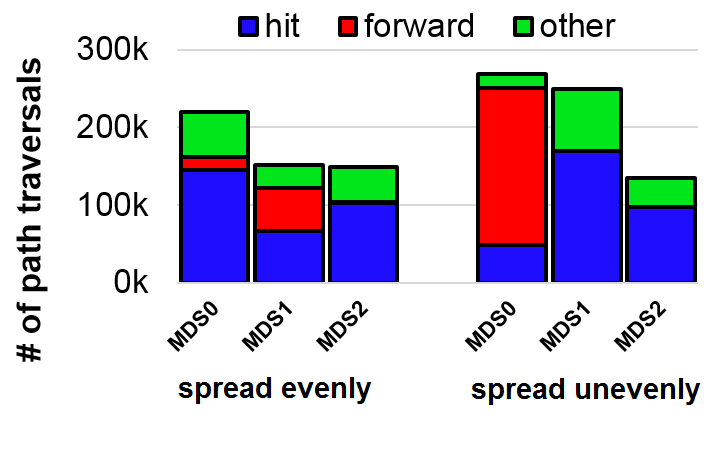
\includegraphics[width=1\textwidth]{./chapters/mantle/figures/workload-tar-traverses2.png}
	\end{subfigure}	
	\caption{Spreading metadata to multiple MDS nodes hurts performance (``spread evenly/unevenly" setups in Figure 3a) when compared to keeping all metadata on one MDS (``high locality'' setup in Figure 3a). The times given are the total times of the job (compile, read, write, etc.). Performance is worse when metadata is spread unevenly because it ``forwards" more requests (Figure 3b).\label{figure:workload-tar-requests}}
\end{figure*}

% Distribution hurts performance
Distributing metadata for balance tries to spread metadata evenly across the metadata cluster. The advantage of this approach is that clients can contact different servers for their metadata in parallel. Many metadata balancers distribute metadata for complete balance by hashing a unique identifier, like the inode or filename; unfortunately, with such fine grain distribution, locality is completely lost. Distributing for locality keeps related metadata on one MDS and can improve performance. The reasons are discussed in ~\cite{weil:phdthesis07, weil:sc2004-dyn-metadata}, but briefly, improving locality can: 
\begin{itemize}
	\item reduce the number of forwards between MDS nodes ({\it i.e.} requests for metadata outside the MDS node's jurisdiction)
	\item lower communication for maintaining coherency ({\it i.e.} requests involving prefix path traversals and permission checking)
	\item reduce the amount of memory needed to cache path prefixes. If metadata is spread, the MDS cluster replicates parent inode metadata so that path traversals can be resolved locally
\end{itemize}

% Example
Figure~\ref{figure:workload-tar-requests} alters the degree of locality by changing how metadata is distributed for a client compiling code on CephFS; with less locality, the performance gets worse and the number of requests increases. The number of requests ({\it y} axis) increases when metadata is distributed: the ``high locality" bar is when all metadata is kept on one MDS, the ``spread evenly" bar is when hot metadata is correctly distributed, and the ``spread unevenly" bar is when hot metadata is incorrectly distributed\footnote{To get high locality, all metadata is kept on one MDS. To get different degrees of spread, we change the setup: ``spread unevenly'' is untarring and compiling with 3 MDS nodes and ``spread evenly'' is untarring with 1 MDS and compiling with 3 MDS nodes. In the former, metadata is distributed when untarring (many creates) and the workload loses locality.}. For this example, the speedup for keeping all metadata on a single MDS is between 18\% and 19\%. Although this is a small experiment, where the client clearly does not overload one MDS, it demonstrates how unnecessary distribution can hurt performance.

% Reason for improvement in performance
The number of requests increases when distributing metadata because the MDS nodes need to forward requests for remote metadata in order to perform common file system operations. The worse the distribution and the higher the fragmentation, the higher the number of forwards. Figure~\ref{figure:workload-tar-traverses} shows that a high number of path traversals ({\it y} axis) end in "forwards" to other MDS nodes when metadata is spread unevenly. When metadata is spread evenly, much more of the path traversals can be resolved by the current MDS ({\it i.e.} they are cache "hits"). Aggressively caching all inodes and prefixes can reduce the requests between clients and MDS nodes, but CephFS (as well as many other file systems) do not have that design, for a variety of reasons.

%%%%%%%%%%%%%%%%%%%%%%%%%%%%%%%%%%%%%%%%%%%%%%%%%%%%%%%%%%%%%%%%%%
\subsection{Multi-MDS Challenges}					    %%%%%%%%%%
\label{multi-mds_challenges}						    %%%%%%%%%%
%%%%%%%%%%%%%%%%%%%%%%%%%%%%%%%%%%%%%%%%%%%%%%%%%%%%%%%%%%%%%%%%%%
% ACTION ITEM: survey paper of load balancing
Dynamic subtree partitioning achieves varying degrees of locality and distribution by changing the way it carves up the namespace and partitions the cluster. To alleviate load quickly, dynamic subtree partitioning can move different sized resources (inodes) to computation engines with variable capacities (MDS nodes), but this flexibility has a cost. In the sections below, we describe CephFS's current architecture and demonstrate how its complexity limits performance. While this section may seem like an argument against dynamic subtree partitioning, our main conclusion is that the approach has potential and warrants further exploration. 

%%%%%%%%%%%%%%%%%%%%
\subsubsection{Complexity Arising from Flexibility}
\label{complexity-arising-from-flexibility}
%%%%%%%%%%%%%%%%%%%%

% The problem: load balancing is hard
The complexity of deciding where to migrate resources increases significantly if these resources have different sizes and characteristics. To properly balance load, the balancer must model how components interact. First, the model needs to be able to predict how different decisions will positively impact performance. The model should consider what can be moved and how migration units can be divided or combined. It should also  consider how splitting different or related objects affects performance and behavior. Second, the model must quantify the state of the system using available metrics. Third, the model must tie the metrics to the global performance and behavior of the system. It must consider how over-utilized resources negatively affect performance and how system events can indicate that the system is performing optimally. With such a model, the balancer can decide which metrics to optimize for.

% Basic overview of cluster and workloads
Figure~\ref{figure:creates-thruput} shows how a 10 node, 3 MDS CephFS system struggles to build an accurate model that addresses the challenges inherent to the metadata management problem. That figure shows the total cluster throughput ({\it y} axis) over time ({\it x} axis) for 4 runs of the same job: creating 100,000 files in separate directories. The top graph, where the load is split evenly, is what the balancer tries to do. The results and performance profiles of the other 3 runs demonstrate that the balancing behavior is not reproducible, as the finish times vary between 5 and 10 minutes and the load is migrated to different servers at different times in different orders. Below, we discuss the design decisions that CephFS made and we demonstrate how policies with good intentions can lead to poor performance and unpredictability.

% /user/msevilla/results/multimds/3mds-3client-sepdir/graphs/images/create-throughput_run5.pdf
\begin{figure}[tb]
	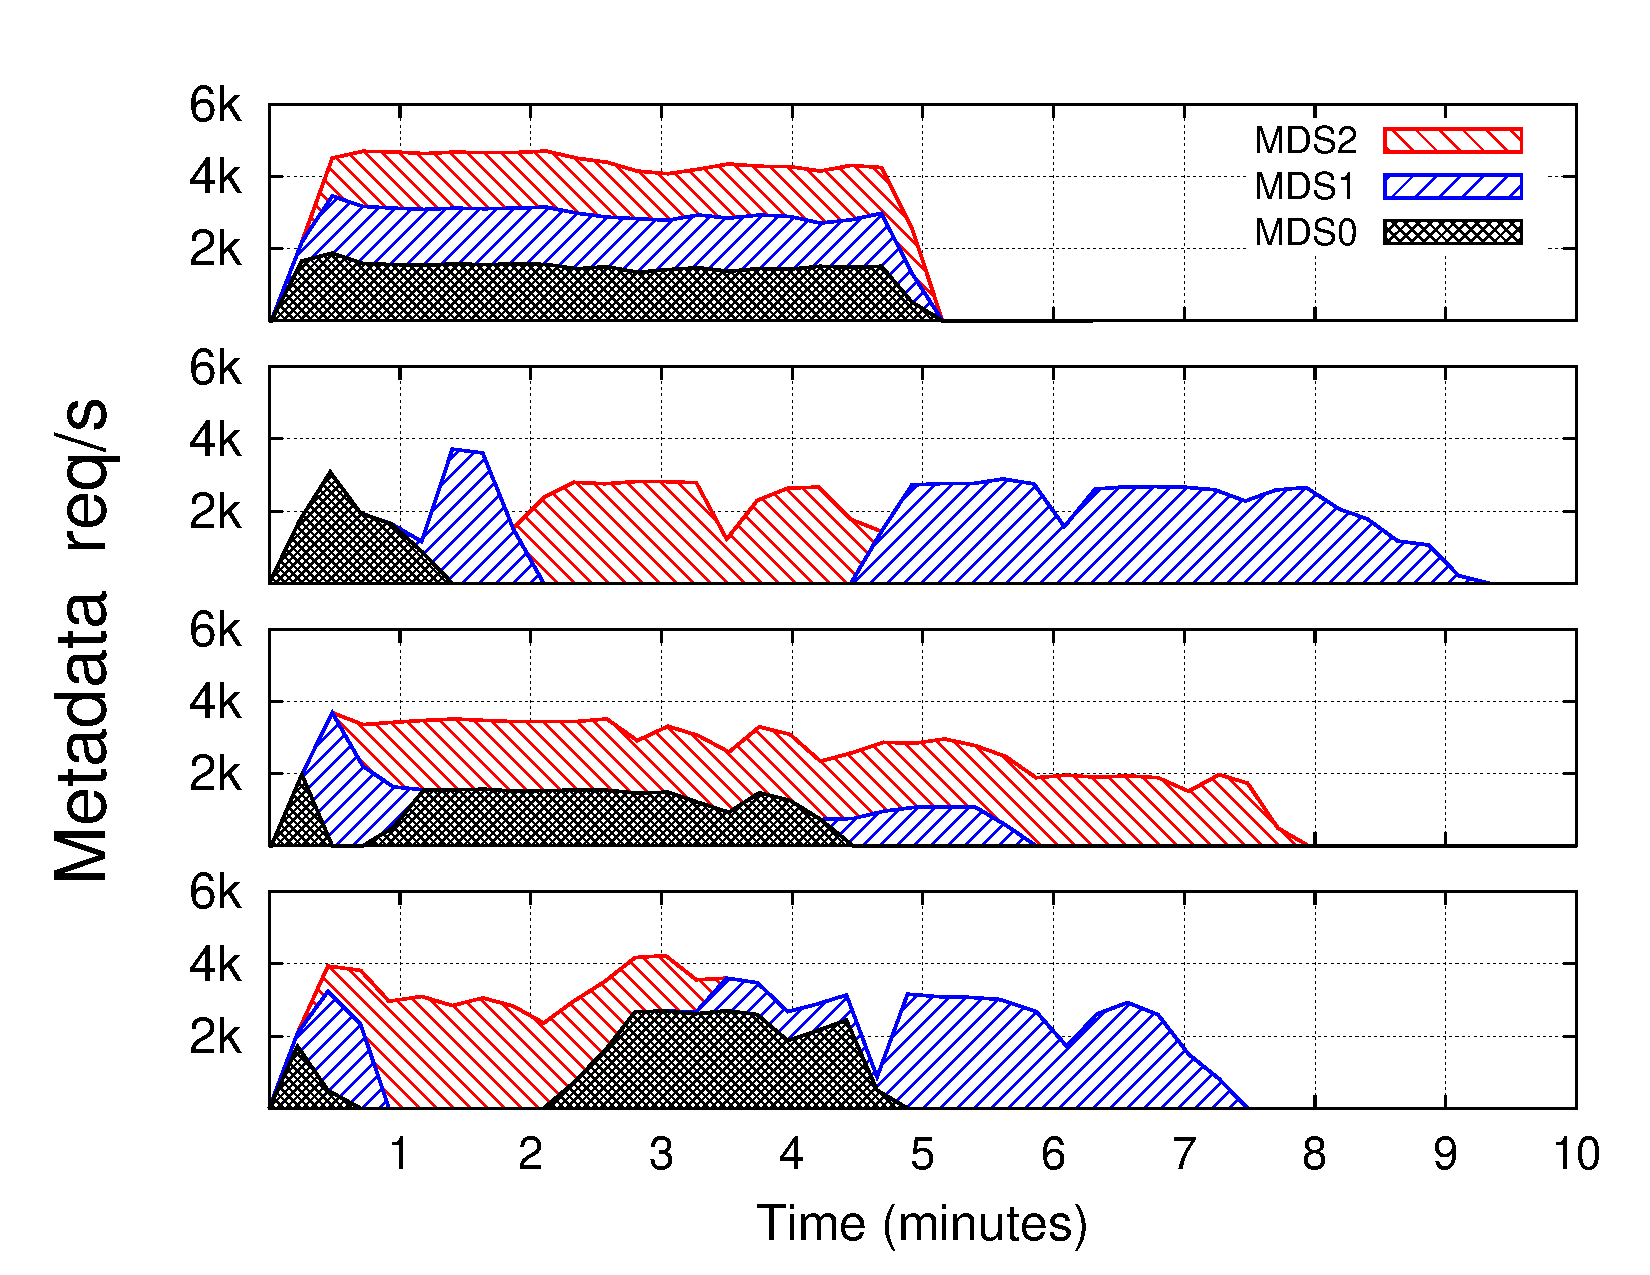
\includegraphics[width=0.45\textwidth]{./chapters/mantle/figures/creates-thruput-runs2.pdf}
	\caption{The same create-intensive workload has different throughput ({\it y} axis; curves are stacked) because of how CephFS maintains state and sets policies.\label{figure:creates-thruput}}
\end{figure}
%%%%%%%%%%%%%%%%%%%%
\subsubsection{Maintaining Global \& Local State}
\label{the-challenge-in-maintaining_global_local_state}
%%%%%%%%%%%%%%%%%%%%

To make fast decisions, CephFS measures, collects, and communicates small amounts of state. Each MDS runs its balancing logic concurrently - this allows it to construct its own view of the cluster. The design decisions of the current balancer emphasizes speed over accuracy: 
\begin{enumerate}
	\item \textbf{Instantaneous measurements}: this makes the balancer sensitive to common system perturbations. The balancer can be configured to use CPU utilization as a metric for making decisions but this metric depends on the instant the measurement is taken and can be influenced by the measurement tool. The balancer dulls this effect by comparing the current measurement against the previous measurement, but in our experiences decisions are still made too aggressively. 
	\item \textbf{Decentralized MDS state}: this makes the balancers reliant on state that is slightly stale. CephFS communicates the load of each MDS around the cluster using heartbeats, which take time to pack, travel across the network, and unpack. As an example, consider the instant MDS0 makes the decision to migrate some of its load; at this time, that MDS considers the aggregate load for the whole cluster by looking at all incoming heartbeats, but by the time MDS0 extracts the loads from all these heartbeats, the other MDS nodes have already moved on to another task. As a result of these inaccurate and stale views of the system, the accuracy of the decisions varies and reproducibility is difficult. 
\end{enumerate}

Even if maintaining state was instant and consistent, making the correct migration decisions would still be difficult because the workload itself constantly changes.

%%%%%%%%%%%%%%%%%%%%
\subsubsection{Setting Policies for Migration Decisions}
\label{setting-policies-for-migration-decisions}
%%%%%%%%%%%%%%%%%%%%
\begin{table}[tb]
	\centering
	\begin{tabular}{ >{}p{1.5cm} | >{}p{6.8cm}}
		\centering\textbf{Policy} & \centering\textbf{Hard-coded implementation}
		\tabularnewline\hline		
		metaload	 	& \small{\texttt{= inode reads + 2*(inode writes)}}\tabularnewline
					 	& \small{\texttt{~~+ read dirs + 2*fetches + 4*stores}}\tabularnewline        
		MDSload      	& \small{\texttt{= 0.8*(metaload on auth)}}\tabularnewline
        				& \small{\texttt{~~+ 0.2*(metaload on all)}}\tabularnewline
        				& \small{\texttt{~~+ request rate + 10*(queue length)}}\tabularnewline
		when			& \small{\texttt{if my load \(>\) (total load)/\#MDSs}}\tabularnewline
        
		where			& \small{\texttt{for each MDS}}\tabularnewline	
          			& \small{\texttt{~~if load > target:add MDS to exporters}}
		\tabularnewline	& \small{\texttt{~~else:add MDS to importers}}
		\tabularnewline	& \small{\texttt{match large importers to large exporters}}\tabularnewline	
        
		how-much 		& \small{\texttt{for each MDS}}\tabularnewline
        accuracy		& \small{\texttt{~~while load already sent < target load}} \tabularnewline
        				& \small{\texttt{~~~~export largest dirfrag}}\tabularnewline
	\end{tabular}	
   	\caption{In the CephFS balancer, the policies are tied to mechanisms: loads quantify the work on a subtree/MDS; when/where policies decide when/where to migrate by assigning target loads to MDS nodes; how-much accuracy is the strategy for sending dirfrags to reach a target load.\label{table:policies}}    
\end{table}	

% Tunables
In complicated systems there are two approaches for setting policies to guide decisions: expose the policies as tunable parameters or tie policies to mechanisms. Tunable parameters, or tunables, are configuration values that let the system administrator adjust the system for a given workload. Unfortunately, these tunable parameters are usually so specific to the system that only an expert can properly tune the system. For example, Hadoop version 2.7.1 exposes 210 tunables to configure even the simplest MapReduce application. CephFS has similar tunables. For example, the balancer  will not send a dirfrag with load below \texttt{mds\_bal\_need\_min}. Setting a sensible value for this tunable is almost impossible unless the administrator understands the tunable and  has an intimate understanding of how load is calculated.

% Tie mechanism to policy
The other approach for setting policies is to hard-code the policies into the system alongside the mechanisms. This reduces the burden on the system administrator and lets the developer, someone who is very familiar with the system, set the policies. 

%%%%%%%%%%%%%%%%%%%%
\subsubsection*{The CephFS Policies}
\label{the-cephfs-policies}
%%%%%%%%%%%%%%%%%%%%
% /user/msevilla/results/1mds/sepdir/graphs/images/create-latency-throughput.pdf
\begin{figure}[tb]
	\centering
	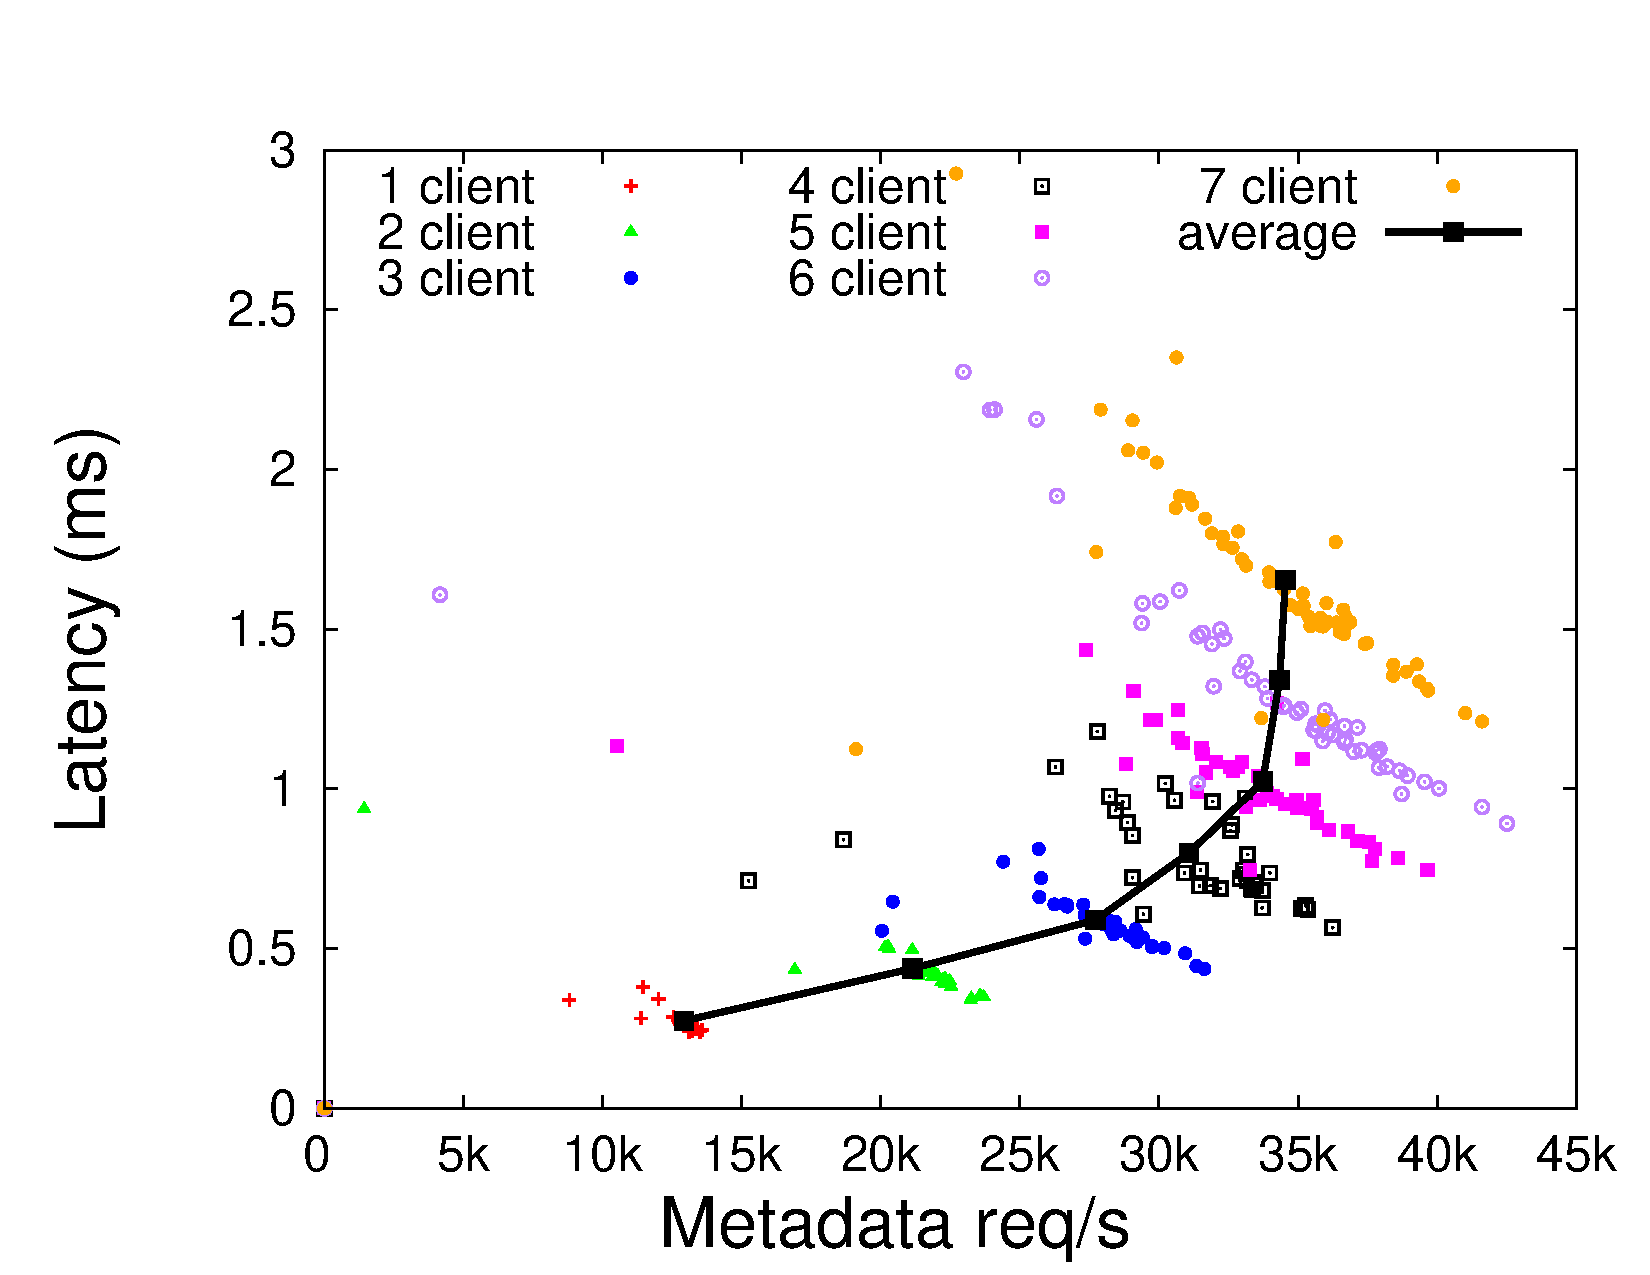
\includegraphics[width=0.45\textwidth]{./chapters/mantle/figures/creates-latency-thruput-clients.pdf}
    \caption{For the create heavy workload, the throughput ({\it x} axis) stops improving and the latency ({\it y} axis) continues to increase with 5, 6, or 7 clients. The standard deviation also increases for latency (up to 3\(\times\)) and throughput (up to 2.3\(\times\)). \label{figure:creates-latency-thruput-clients}} 
\end{figure}

% scalarization 
The CephFS policies, shown in Table~\ref{table:policies}, shape decisions using two techniques: scalarization of logical/physical metrics and hard-coding the logic. Scalarization means collapsing many metrics into a single value, usually with a weighted sum. When partitioning the cluster and the namespace, CephFS calculates metadata and MDS loads by collapsing the logical ({\it e.g.,} inode reads, inode writes, readdirs, etc.) and physical metrics ({\it e.g.,} CPU utilization, memory usage, etc.) into a single value. The exact calculations are in the ``metaload" and ``MDS load'' rows of Table~\ref{table:policies}. 

% Hard code
The other technique CephFS uses in its policies is to compile the decision logic into the system. The balancer uses one approach for deciding when and where to move inodes; it migrates load when it thinks that it has more load than the other MDS nodes (``when" row of Table~\ref{table:policies}) and it tries to migrate enough of its load to make the load even across the MDS cluster (``where" row of Table~\ref{table:policies}). While this approach is scalable, it reduces the efficiency of the cluster if the job could have been completed with less MDS nodes. Figure~\ref{figure:creates-latency-thruput-clients} shows how a single MDS performs as the number of clients is scaled, where each client is creating 100,000 files in separate directories. With an overloaded MDS servicing 5, 6, or 7 clients, throughput stops improving and latency continues to increase. With 1, 2, and 3 clients, the performance variance is small, with a standard deviation for latency between 0.03 and 0.1 ms and for throughput between 103 and 260 requests/second; with 3 or more clients, performance is unpredictable, with a standard deviation for latency between 0.145 and 0.303 ms and for throughput between 406 and 599 requests/second. This indicates that a single MDS can handle up to 4 clients without being overloaded.

% How we can explore accuracy vs. quickness
Each balancer also sets policies for shedding load from its own namespace.  While partitioning the cluster, each balancer assigns each MDS a target load, which is the load the balancer wants to send to that particular MDS. The balancer starts at its root subtrees and continuously sends the largest subtree or dirfrag until reaching this target load (``how-much accuracy" row of Table~\ref{table:policies}). If the target is not reached, the balancer ``drills" down into the hierarchy. This heuristic can lead to poor decisions. For example, in one of our create heavy runs we had 2 MDS nodes, where MDS0 had 8 ``hot" directory fragments with metadata loads: 12.7, 13.3, 13.3, 14.6, 15.7, 13.5, 13.7, 14.6. The balancer on MDS0 tried to ship off half the load by assigning MDS1 a target load of:
\(\frac{\text{total load}}{\text{\# MDSs}} = 55.6\). 
To account for the noise in load measurements, the balancer also scaled the target load by 0.8 (the value of the \texttt{mds\_bal\_need\_min} tunable). As a result, the balancer only shipped off 3 dirfrags, 15.7 + 14.6 + 14.6, instead of half the dirfrags. 

% Why this is set
It is not the case that the balancer cannot decide how much load to send; it is that the balancer is limited to one heuristic (biggest first) to send off dirfrags. We can see why this policy is chosen; it is a fast heuristic to address the bin-packing problem (packing dirfrags onto MDS nodes), which is a combinatorial NP-Hard problem. This approach optimizes the speed of the calculation instead of accuracy and, while it may work for large directories with millions of entries, it struggles with simpler and smaller namespaces because of the noise in the load measurements and calculations.


